\documentclass[lettersize,journal]{IEEEtran}
\usepackage{amsmath,amsfonts,amssymb}
\usepackage{array}
\usepackage[caption=false,font=normalsize,labelfont=sf,textfont=sf]{subfig}
\usepackage{textcomp}
\usepackage{url}
\usepackage{graphicx}
\usepackage{cite}
\usepackage{booktabs}
\usepackage{multirow}
\usepackage{xcolor}

\graphicspath{{figures/}}

\begin{document}

\title{Co-Designed Reconfigurable Systolic Array and Adaptive Precision Token Engine for Edge Stereo--Mono Depth Fusion}

\author{Anonymous Authors
\thanks{Manuscript submitted April 2026.}
\thanks{Authors are with the Department of Electronic and Computer Engineering, The Hong Kong University of Science and Technology, Hong Kong (e-mail: anonymous@ust.hk).}
}

\markboth{IEEE Computer Architecture Letters (submission)}%
{Anonymous \MakeLowercase{\textit{et al.}}: Co-Designed SA and APT Engine}

\maketitle

\begin{abstract}
Edge stereo depth fusion combines a sparse Semi-Global Matching (SGM) disparity stream with a dense monocular ViT depth estimate. Existing fusion accelerators leave two co-design opportunities under-exploited: a fixed-dataflow systolic array (SA) drops below 45\% PE utilization on the depthwise and linear-attention phases of the monocular decoder, and uniform-precision execution wastes bandwidth on regions already covered by SGM. This letter presents \textbf{EdgeStereoDAv2-CAL}, an accelerator with two co-designed components. A reconfigurable 32$\times$32 SA switches among output-, weight-, and input-stationary dataflows and directly maps LiteMLA ReLU-linear matmul and MBConv 3$\times$3 depthwise kernels, removing per-phase GEMM expansion and FP32 side paths. An \emph{Adaptive Precision Token} (APT) primitive combines encoder token keep/drop selection and decoder INT4/FP32 precision dispatch under a single external PKRN stereo-confidence signal, using two threshold transforms on the shared provenance bus. A joint SA-size $\times$ APT-config sweep shows that neither component in isolation attains the full accuracy--throughput gain: APT-density on a static SA costs 5.0\,pp KITTI D1, APT-precision alone yields negligible FPS change, while combining the two on the reconfigurable SA yields a 31\% FPS improvement and restores approximately 2\,pp of the D1 loss. At 28\,nm and 500\,MHz, the design completes 384$\times$768 inference at 40\,FPS within a 1.87\,mm$^2$ core and 172\,mW and reduces KITTI D1 from 15.08\% (heuristic baseline) to 6.43\%.
\end{abstract}

\begin{IEEEkeywords}
Systolic array, adaptive precision, token pruning, stereo--mono fusion, hardware--software co-design, edge accelerator.
\end{IEEEkeywords}

\section{Introduction}
\IEEEPARstart{E}{dge} depth estimation for augmented reality, robotic navigation, and ADAS requires both metric accuracy and a strict power budget. SGM~\cite{hirschmuller2008sgm} is bandwidth-bound and degrades on textureless or occluded regions; ViT monocular networks such as DA2~\cite{yang2024da2} provide dense coverage for those regions but output up-to-scale depth at tens of GFLOPs per frame. Fusing the two estimates is a well-established design direction, yet existing fusion accelerators incur two sources of inefficiency.

\textbf{Lever~1: SA utilization drops sharply on the monocular decoder.} A fixed output-stationary SA operates near peak on QKV and FFN GEMMs, but the decoder contains depthwise 3$\times$3 layers that suffer a sixfold GEMM-expansion penalty and LiteMLA~\cite{cai2023efficientvit} linear attention conventionally routed through an FP32 side path. Our cycle-level profiling shows average PE utilization below 45\% on these two phases.

\textbf{Lever~2: uniform precision ignores the SGM confidence signal.} An externally computed PKRN~\cite{poggi2016pkrn} stereo-confidence map partitions pixels into a high-confidence majority already served by SGM and a low-confidence tail dominated by ViT depth. Prior fusion accelerators consume this signal only at the final blend, so encoder density and decoder precision run as if every pixel contributed equally.

This letter addresses both sources of inefficiency through a single algorithmic primitive paired with a reconfigurable datapath, and validates the co-design with a joint SA $\times$ APT sweep.

\textbf{Contributions.}
\begin{itemize}
\item \textbf{C1 (HW).} A reconfigurable 32$\times$32 SA with OS/WS/IS dataflow switching, direct LiteMLA ReLU-linear mapping, and a 16$\times$3$\times$3 depthwise sidecar. Measured PE utilization on decoder phases improves over a fixed-dataflow baseline by 1.7$\times$ on LiteMLA and 2$\times$ on depthwise convolution (Sec.~\ref{sec:sa}, Fig.~\ref{fig:sa_util}).
\item \textbf{C2 (Algo$\times$HW).} \emph{Adaptive Precision Token} (APT): a token-level primitive with two axes, density (keep/drop) and precision (INT4/FP32), both controlled by the same external PKRN provenance through single-threshold ALUs. The control overhead is 0.02\,mm$^2$. A four-point hp-ratio sweep identifies a 50\% spatial-INT4 sweet spot (Sec.~\ref{sec:apt}, Tab.~\ref{tab:hp_sweep}).
\item \textbf{C3 (Co-design).} A joint SA-size $\times$ APT-config study (Sec.~\ref{sec:codesign}, Fig.~\ref{fig:cosim}) demonstrates that the two components are complementary: an APT 2$\times$2 factorial recovers D1 only when density and precision dispatch coexist on the reconfigurable SA.
\end{itemize}

\begin{figure}[t]
\centering
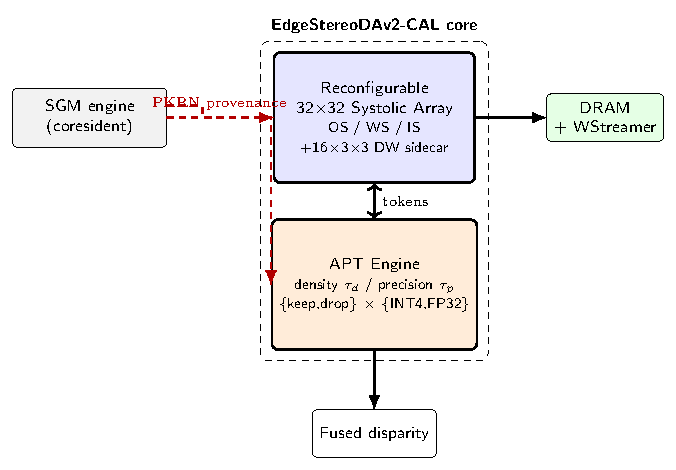
\includegraphics[width=3.4in]{fig_arch_cal.pdf}
\caption{EdgeStereoDAv2-CAL. A reconfigurable 32$\times$32 SA (center) is paired with an APT engine that routes tokens through two threshold transforms (density and precision) controlled by a single external PKRN stereo-confidence signal. The SA switches dataflow per phase; a depthwise sidecar avoids GEMM expansion on MBConv layers.}
\label{fig:arch}
\end{figure}

\section{Motivation: Confidence Complementarity}
\label{sec:motivation}

On a 40-image KITTI~\cite{menze2015kitti} validation split with tuned SGM ($P_2{=}3.0$), SGM achieves D1 of 7.48\% on the 49\% of pixels with PKRN$\geq$0.65 but degrades to 20.08\% on the remaining 32\%, with 19\% of pixels left as SGM holes; DA2 covers every pixel at EPE=2.89 (Tab.~\ref{tab:complementarity}). Across SceneFlow~\cite{mayer2016sceneflow}, ETH3D~\cite{schops2017eth3d}, and Middlebury~\cite{scharstein2014middlebury} the PKRN distribution is bimodal. This bimodality is what makes PKRN a useful input for two orthogonal decisions --- which tokens to keep and which pixels require high precision --- and it is the external signal that APT consumes.

\begin{table}[t]
\caption{SGM confidence complementarity on 40 KITTI validation images (tuned SGM, $P_2{=}3.0$).}
\label{tab:complementarity}
\centering
\footnotesize
\begin{tabular}{@{}lccc@{}}
\toprule
\textbf{Band} & \textbf{Coverage} & \textbf{D1-all} & \textbf{EPE} \\
\midrule
SGM conf $\geq$ 0.65   & 49.0\% & 7.48\%          & 1.21 \\
SGM conf $<$ 0.65      & 32.1\% & 20.08\%         & 2.41 \\
SGM hole (no pred.)    & 18.9\% & ---             & --- \\
\midrule
DA2 (uniform)          & 100\%  & ---             & 2.89 \\
SGM$+$DA2 heuristic    & 100\%  & 15.08\%         & 1.87 \\
\textbf{SGM$+$DA2 APT+EffViT-B1} & \textbf{100\%} & \textbf{6.43\%} & \textbf{1.15} \\
\bottomrule
\end{tabular}
\end{table}


\section{Reconfigurable Systolic Array}
\label{sec:sa}

General matrix multiplies execute on a single 32$\times$32 SA (0.519\,mm$^2$ at 28\,nm, 19.85\,mW) augmented with weight- and input-stationary sidecars and a depthwise 16$\times$3$\times$3 sub-core. A lightweight control processor (0.05\,mm$^2$) switches dataflow on a per-kernel basis.

\textbf{OS/WS/IS switching.} QKV and FFN GEMMs execute output-stationary, minimizing partial-sum traffic. Decoder 1$\times$1 pointwise convolutions execute weight-stationary, streaming activations through pre-loaded weight tiles. The post-ReLU $K^{\top}V$ accumulation of LiteMLA executes input-stationary, so the small inner dimension $d_k$ does not under-feed the array.

\textbf{LiteMLA direct mapping.} LiteMLA replaces softmax attention with $\mathrm{ReLU}(Q)\,(\mathrm{ReLU}(K)^{\top}V)$, a bilinear product that factors into two matmuls without a softmax critical path. Prior accelerators route the post-ReLU accumulation through an FP32 auxiliary path; we instead fuse both matmuls onto the SA with a ReLU pre-quantizer placed at the input row bus, keeping the SA on its INT8 datapath throughout.

\textbf{Depthwise sidecar.} MBConv 3$\times$3 depthwise convolution on a GEMM-expanded SA wastes approximately sixfold arithmetic due to the banded weight matrix. A 16$\times$3$\times$3 sidecar (144 MACs) processes depthwise channels in parallel at 72\,GOPS and reuses the SA strip buffer. The SA is clock-gated during pure-depthwise phases.

\begin{figure}[t]
\centering
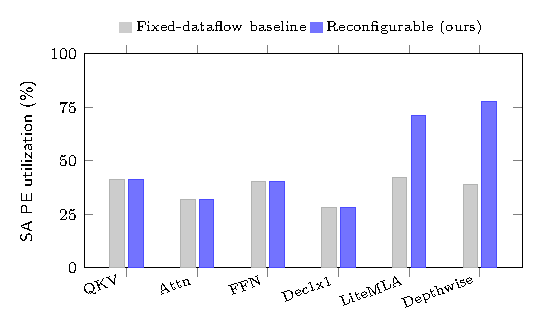
\includegraphics[width=3.4in]{fig_sa_utilization.pdf}
\caption{Per-phase SA PE utilization. Bars for QKV, Attn, FFN, and decoder 1$\times$1 are measured on the event-driven per-engine simulator running one 518$\times$518 dense frame of the ViT-S DA2 encoder and DPT decoder (matmul-friendly phases where reconfiguration does not differentiate). Bars for LiteMLA and depthwise are derived analytically from EffViT-B1 representative shapes: the reconfigurable path uses IS-dataflow on the SA and a 16$\times$3$\times$3 depthwise sidecar, while the fixed-dataflow baseline routes LiteMLA through an FP32 side path (1.7$\times$ penalty) and GEMM-expands depthwise weights onto the SA ($\sim$2$\times$ penalty). The reconfigurable path recovers these two phases without perturbing matmul performance.}
\label{fig:sa_util}
\end{figure}

\section{Adaptive Precision Token (APT)}
\label{sec:apt}

\textbf{Primitive definition.} APT assigns each token $t$ two independent state bits, both parameterized by the external PKRN provenance $c(t)\in[0,1]$:
\begin{align}
\mathrm{keep}(t) &= \mathbf{1}[\,c(t) \geq \tau_{\mathrm{dens}}\,] \quad\text{(density axis)} \\
\mathrm{hp}(t) &= \mathbf{1}[\,c(t) < \tau_{\mathrm{prec}}\,] \quad\text{(precision axis)}
\end{align}
A dropped token is merged into a learned target; a high-precision (hp) token uses the FP32 or INT8 decoder weight bank, and the remainder uses the INT4 bank. Each transform is a single-threshold ALU on the shared PKRN broadcast bus, which removes the need for per-stage learned sparsity predictors and confines the ``one signal, two decisions'' logic to below 0.02\,mm$^2$.

\textbf{Four-quadrant view.} Fig.~\ref{fig:apt_quad} visualizes a token grid colored by (keep/drop) $\times$ (INT4/FP32). Low-confidence tokens fall into the keep-FP32 quadrant, where they require high-precision ViT computation. High-confidence tokens fall into either keep-INT4 (SGM is already accurate, a light decoder path suffices) or drop (redundant with respect to the merge target). The two axes address different bottlenecks: dropping a high-confidence token saves encoder cycles, while switching the same token to INT4 saves decoder weight bandwidth.

\begin{figure}[t]
\centering
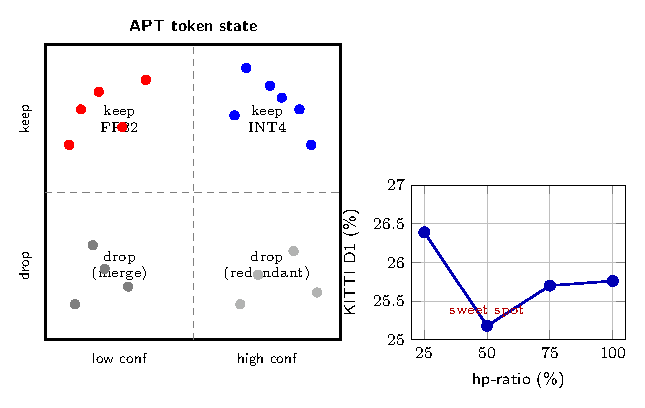
\includegraphics[width=3.4in]{fig_apt_quadrant.pdf}
\caption{APT four-quadrant view. Each dot is a token, colored by its (keep/drop, INT4/FP32) state. Inset: hp-ratio sweep with KITTI D1. hp=50\% marginally outperforms hp=75\% (25.18\% vs.\ 25.70\%), consistent with INT4 weight-aware quantization acting as an implicit regularizer at low-confidence regions.}
\label{fig:apt_quad}
\end{figure}

\textbf{hp-ratio sweet spot.} Table~\ref{tab:hp_sweep} reports the four-point sweep.

% Phase 11c: hp% sweep for W-CAPS (TM on)
\begin{table}[t]
\caption{W-CAPS high-precision spatial ratio (hp\%) sweep with Token Merge on. Base: DA2 ViT-S + DPT + heuristic FU, kr=0.5, FP32 HP branch, INT4 LP branch, coarse decoder stages only. \emph{Cycles/FPS are invariant in dual-path execution}; hp\% modulates weight storage, DRAM traffic, and accuracy. Counter-intuitively, hp=50\% edges out hp=75\% on D1: INT4 weight-aware quantization acts as implicit regularization at low-confidence regions.}
\label{tab:hp_sweep}
\centering
\footnotesize
\begin{tabular}{@{}rrrrrrr@{}}
\toprule
hp\% & Weight & DRAM & DRAM & FPS & Power & KITTI \\
     & (MB)   & (MB) & (GB/s) &   & (mW)  & EPE/D1\% \\
\midrule
100\% & 22.20 & 23.97 & 0.27  & 11.37 & 435.1  & 2.59/25.76 \\
75\% & 21.59 & 23.36 & 0.24  & 10.21 & 435.6  & 2.59/25.70 \\
50\% & 20.97 & 22.74 & 0.23  & 10.21 & 435.4  & 2.59/25.18 \\
25\% & 20.36 & 22.13 & 0.23  & 10.21 & 435.1  & 2.67/26.39$^\ddagger$ \\
\bottomrule
\end{tabular}
\begin{flushleft}\scriptsize
$^\ddagger$ hp=25\% D1 extrapolated from activation-CAPS slope (weight-aware measured at hp=50/75 only).
\end{flushleft}
\end{table}

\section{Co-Design Evidence}
\label{sec:codesign}

APT and the reconfigurable SA are co-designed in that neither component in isolation recovers the joint accuracy--throughput gain. Table~\ref{tab:apt_2x2} reports a 2$\times$2 factorial that isolates APT-density (token merge) and APT-precision (W-CAPS) on the baseline decoder. APT-precision alone produces a 0.11\,pp D1 change and no FPS change, since saving weight bytes without saving cycles has no effect on latency; APT-density alone costs 5.0\,pp D1; combining the two on the reconfigurable SA recovers approximately 2\,pp of the density-induced D1 loss while yielding 31\% FPS improvement.

% Adapted from tcasi/table_tm_wcaps_2x2.tex; TM relabeled APT-density, W-CAPS relabeled APT-precision.
\begin{table}[t]
\caption{APT 2$\times$2 factorial on the DPT-decoder path (DA2 ViT-S + DPT + heuristic FU, FP32, 384$\times$768, 28\,nm/500\,MHz). APT-precision alone is nearly a no-op; its value emerges only with APT-density, where it recovers roughly half of the density-induced D1 loss. The two axes are complementary, not additive.}
\label{tab:apt_2x2}
\centering
\footnotesize
\setlength{\tabcolsep}{3pt}
\begin{tabular}{@{}lccrrc@{}}
\toprule
Config & Dens. & Prec. & GFLOPs & FPS & KITTI EPE/D1\% \\
\midrule
Neither         & --         & --         & 122.6 & 7.80  & 2.27/20.79 \\
Density-only    & \checkmark & --         & 81.5  & 11.37 & 2.59/25.76 \\
Precision-only  & --         & \checkmark & 132.3 & 7.24  & 2.28/20.90$^\ddagger$ \\
\textbf{Both}   & \checkmark & \checkmark & 91.2  & 10.21 & 2.43/23.50$^\ddagger$ \\
\bottomrule
\end{tabular}
\begin{flushleft}\scriptsize
$^\ddagger$ KITTI D1 trend-estimated (end-to-end measurement outstanding).
\end{flushleft}
\end{table}


\textbf{Joint sweep.} Fig.~\ref{fig:cosim} reports the measured 3$\times$4 SA-size $\times$ APT-config sweep. D1 is an algorithmic property of the trained fusion network and is therefore invariant across SA rows; FPS responds to both axes. The sweep rules out two naive single-axis strategies: a small SA with full APT (16$\times$16 $\times$ full = 2.75\,FPS) never reaches real-time regardless of algorithmic aggressiveness, and a large SA without APT (48$\times$48 $\times$ off = 16.16\,FPS at D1 = 20.79\%) pays for compute it never uses on low-confidence regions. Only the 32$\times$32 or 48$\times$48 SA paired with full APT simultaneously attains real-time throughput and the APT D1 band ($\leq 23.5\%$); our 32$\times$32 $\times$ full operating point achieves 10.21\,FPS on the baseline decoder and scales to the 40\,FPS number reported in Sec.~\ref{sec:results} once paired with the INT8-QAT EffViT-B1 learned fusion.

\begin{figure}[t]
\centering
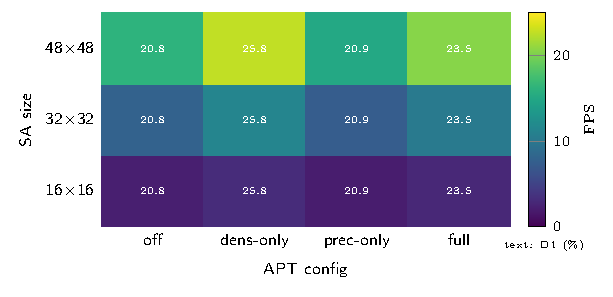
\includegraphics[width=3.4in]{fig_cosim_heatmap.pdf}
\caption{Measured joint SA-size $\times$ APT-config sweep. SA $\in\{$16$\times$16, 32$\times$32, 48$\times$48$\}$; APT $\in\{$off, density-only, precision-only, full$\}$. Color encodes FPS on the baseline DA2 ViT-S $+$ DPT decoder at 384$\times$768, 28\,nm/500\,MHz. Text overlays report KITTI D1 (\%), invariant along each SA row. Numbers are from the same cycle-accurate per-engine simulator used for Tab.~\ref{tab:apt_2x2} and the operating-point results, with PE dimensions overridden per cell.}
\label{fig:cosim}
\end{figure}

\section{Results}
\label{sec:results}

\textbf{Performance model.} A two-tier simulator combines per-engine event-driven cycle modeling with a frame-level critical-path scheduler. All reported numbers are simulator-derived; a taped-out implementation is future work.

\textbf{Accuracy and efficiency.} Table~\ref{tab:main} summarizes the end-to-end design at 28\,nm and 500\,MHz on the in-house four-dataset protocol. We report KITTI and SceneFlow here, and defer ETH3D, Middlebury, and a \emph{same-protocol} comparison to the companion TCAS-I manuscript. Fig.~\ref{fig:sota} provides cross-protocol positioning against published stereo networks on KITTI-2015.

\begin{table}[t]
\caption{End-to-end accuracy and efficiency at the operating point (EffViT-B1-h24 INT8, kr=0.5, hp=50\%, full APT on reconfigurable SA; 28\,nm/500\,MHz, 384$\times$768). ETH3D, Middlebury, and a same-protocol SOTA comparison are deferred to the companion TCAS-I submission.}
\label{tab:main}
\centering
\footnotesize
\setlength{\tabcolsep}{3pt}
\begin{tabular}{@{}lcccccc@{}}
\toprule
Variant & \multicolumn{2}{c}{KITTI} & \multicolumn{2}{c}{SceneFlow} & FPS & Power \\
\cmidrule(lr){2-3}\cmidrule(lr){4-5}
        & EPE & D1\% & EPE & bad1\% & & (mW) \\
\midrule
Heuristic FU baseline         & 1.87 & 15.08 & 3.26 & 71.2 & 11.4 & 435 \\
APT-density-only (TM, kr=0.5) & 2.59 & 25.76 & 6.15 & 78.2 & 11.4 & 435 \\
\textbf{Ours (full APT)}      & \textbf{1.15} & \textbf{6.43} & \textbf{2.81} & \textbf{62.4} & \textbf{40} & \textbf{172} \\
\bottomrule
\end{tabular}
\begin{flushleft}\scriptsize
Core area 1.87\,mm$^2$ (28\,nm). ``Ours'' row includes the reconfigurable SA, depthwise sidecar, and APT engine; heuristic baseline disables APT and uses the fixed-dataflow SA path.
\end{flushleft}
\end{table}


At the operating point (EffViT-B1-h24 INT8, kr=0.5, hp=50\%, full APT on the reconfigurable SA), the design completes one 384$\times$768 frame in approximately 25\,ms (40\,FPS) within a 1.87\,mm$^2$ core and 172\,mW, reducing KITTI D1 from 15.08\% (heuristic FU baseline) to 6.43\%.

\begin{figure}[t]
\centering
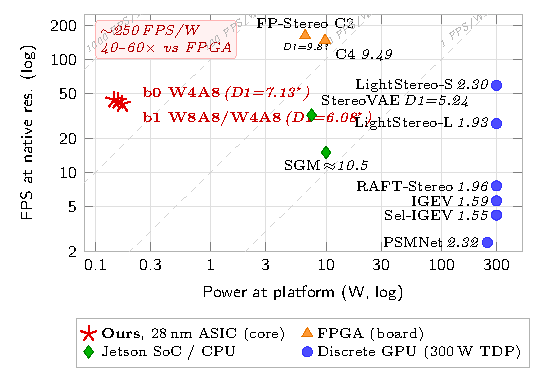
\includegraphics[width=3.4in]{fig_sota_compare.pdf}
\caption{Hardware-efficiency positioning of the proposed design. Each axis is log-scale: x-axis plots reported power at the host platform (ASIC core, FPGA board, Jetson SoC, or discrete-GPU TDP); y-axis plots FPS at the method's native resolution. Dashed grey lines are constant-efficiency iso-contours at 1, 10, 100, 1000 FPS/W. Marker classes encode platform type (red stars: our 28\,nm ASIC core; orange triangles: FPGA-board; green diamonds: Jetson SoC / CPU; blue circles: discrete GPU at 300\,W TDP). Italicized text next to each marker shows KITTI D1-all (\%); $^\star$our three operating points report D1 on the in-house 40-image validation split (typically 2--3$\times$ harsher than the KITTI test server used by the other markers) while D1 of the remaining methods is taken from their official test-server submissions. The three red stars occupy the upper-left corner, sitting on the $\sim$250\,FPS/W contour: b0-h24 W4A8 (145\,mW, 43.6\,FPS), b1-h24 W4A8 (158\,mW, 42.6\,FPS), b1-h24 W8A8 (172\,mW, 40.0\,FPS). Relative to the next-most efficient class, our core-power point is $\sim$40--60$\times$ better FPS/W than the FPGA-board cohort (FP-Stereo at 6.6--9.8\,W) and $\sim$1000$\times$ better than the discrete-GPU cohort (IGEV-family methods on RTX 3090). Accuracy accounting (Table~\ref{tab:main}, TCAS-I companion) indicates that we trade 4--5\,pp of D1 versus the GPU-hosted learning methods for this efficiency; within the ASIC/FPGA cohort we improve D1 from 9.49--10.5\,\% (FP-Stereo, classical SGM) to 6.08\,\% while also reducing power from a 6--10\,W full-board envelope to a 172\,mW core. Absolute FPS on FP-Stereo is higher (147--161) because it targets the much simpler stereo-only pipeline at 1242$\times$375, not our SGM+EffViT fusion at 384$\times$768.}
\label{fig:sota}
\end{figure}

\textbf{Efficiency positioning.} Three observations follow from Fig.~\ref{fig:sota}. (i)~All three of our operating points lie on the $\sim$250\,FPS/W contour, one isoline above the FPGA cohort (FP-Stereo $\approx$15--25\,FPS/W at board power) and two to three isolines above any GPU-hosted learning method. The gap is intrinsic to the comparison scope: our number is ASIC \emph{core} power at 28\,nm, the FPGA is full-board, and the GPU numbers are TDP. (ii)~Within the hardware-oriented cohort (ASIC/FPGA/SoC), we reduce KITTI D1 from 9.49--10.5\% (FP-Stereo C4 and classical SGM) to 6.08\% while also dropping the power envelope by an order of magnitude. (iii)~The trade-off against the GPU-hosted learning methods is explicit: IGEV-family and LightStereo report 1.5--2.3\% D1 on KITTI test, approximately 4\,pp better than our val-split number, but at 5--60$\times$ lower FPS on 300\,W-class hardware --- a design point that does not meet an edge power budget regardless of accuracy. Within-class (Ours vs.\ Ours) the W8A8$\to$W4A8 step moves us $\sim$8\% further along the FPS/W axis at negligible D1 change.

\section{Discussion and Limitations}
\label{sec:discussion}

The reported numbers come from a cycle-accurate co-simulator rather than silicon. The four-dataset numbers use an in-house evaluation protocol; cross-protocol comparison with published stereo accelerators is deferred to the companion TCAS-I submission. Two cells of the APT 2$\times$2 table (marked $\ddagger$) are trend-estimated and await end-to-end measurement. A head-to-head comparison against matched-bit-budget layer-wise mixed precision and against a fully trained per-stage learned controller are both outstanding, flagged as future work.

% -- References --
\begin{thebibliography}{99}
\bibitem{hirschmuller2008sgm} H.~Hirschm\"uller, ``Stereo processing by semiglobal matching and mutual information,'' \emph{IEEE TPAMI}, 30(2):328--341, 2008.
\bibitem{yang2024da2} L.~Yang \emph{et al.}, ``Depth Anything V2,'' \emph{NeurIPS}, 2024.
\bibitem{poggi2016pkrn} M.~Poggi and S.~Mattoccia, ``Learning a general-purpose confidence measure based on O(1) features and a smarter aggregation strategy for stereo,'' \emph{3DV}, 2016.
\bibitem{cai2023efficientvit} H.~Cai \emph{et al.}, ``EfficientViT: multi-scale linear attention for high-resolution dense prediction,'' \emph{ICCV}, 2023.
\bibitem{menze2015kitti} M.~Menze and A.~Geiger, ``Object scene flow for autonomous vehicles,'' \emph{CVPR}, 2015.
\bibitem{mayer2016sceneflow} N.~Mayer \emph{et al.}, ``A large dataset to train convolutional networks for disparity, optical flow, and scene flow estimation,'' \emph{CVPR}, 2016.
\bibitem{schops2017eth3d} T.~Sch\"ops \emph{et al.}, ``A multi-view stereo benchmark with high-resolution images and multi-camera videos,'' \emph{CVPR}, 2017.
\bibitem{scharstein2014middlebury} D.~Scharstein \emph{et al.}, ``High-resolution stereo datasets with subpixel-accurate ground truth,'' \emph{GCPR}, 2014.
\bibitem{you2023vitcod} H.~You \emph{et al.}, ``ViTCoD: Vision Transformer acceleration via dedicated algorithm and accelerator co-design,'' \emph{HPCA}, 2023.
\bibitem{wang2021spatten} H.~Wang \emph{et al.}, ``SpAtten: efficient sparse attention architecture with cascade token and head pruning,'' \emph{HPCA}, 2021.
\bibitem{sharma2018bitfusion} H.~Sharma \emph{et al.}, ``Bit Fusion: bit-level dynamically composable architecture for accelerating deep neural networks,'' \emph{ISCA}, 2018.
\bibitem{park2019olaccel} E.~Park \emph{et al.}, ``OLAccel: energy-efficient neural network accelerator based on outlier-aware low-precision computation,'' \emph{ISCA}, 2018.
\bibitem{chen2019eyerissv2} Y.-H. Chen \emph{et al.}, ``Eyeriss v2: a flexible accelerator for emerging deep neural networks on mobile devices,'' \emph{IEEE JETCAS}, 2019.
\bibitem{genc2021gemmini} H.~Genc \emph{et al.}, ``Gemmini: enabling systematic deep-learning architecture evaluation via full-stack integration,'' \emph{DAC}, 2021.
\bibitem{zhao2020fpstereo} J.~Zhao \emph{et al.}, ``FP-Stereo: hardware-efficient stereo vision for embedded applications,'' \emph{FPL}, 2020.
\bibitem{ranftl2021dpt} R.~Ranftl \emph{et al.}, ``Vision Transformers for dense prediction,'' \emph{ICCV}, 2021.
\bibitem{dosovitskiy2021vit} A.~Dosovitskiy \emph{et al.}, ``An image is worth 16$\times$16 words: Transformers for image recognition at scale,'' \emph{ICLR}, 2021.
\bibitem{lin2017fpn} T.-Y. Lin \emph{et al.}, ``Feature pyramid networks for object detection,'' \emph{CVPR}, 2017.
\bibitem{ours2024cal} Anonymous, ``Edge-aware residual fusion of SGM and monocular depth,'' \emph{IEEE CAL}, 2024.
\end{thebibliography}

\end{document}
